\section{Action Recognition Datasets}
\label{sec:datasets}

\subsection{UCF-101}

All the 13,320 action clips are extracted from 2,500 initial videos.


\subsection{Kinetics}

The training of action recognition systems, which are applicable to the real world, e.g. by adding vision system to robots or by processing existing video streams from cameras heavily relies on the kind and amount of data that is available for training.


\subsection{Charades (Activities of Daily-Living)}

The creation of the Charades dataset \cite{sigurdsson_hollywood_2016} by the Allen Institute of Artificial Intelligence in 2016 addressed common flaws in existing action recognition datasets.
As our earlier survey revealed, publicly available action recognition datasets stem from three common sources:
\begin{enumerate}
    \item Videos are created in controlled environments by filming a finite set of actors performing given actions.
    \item Videos are sampled from movies or television broadcasts, and then labeled either manually or using video-metadata.
    \item Videos are gathered from the internet, i.e. from video platforms such as YouTube.
\end{enumerate}

Datasets from (1.) usually lack the desired variety needed for enabling proper generalization of machine learning approaches and are comparably small, due to the cost of capturing and labeling such data through a single institution.

Datasets from (2.) and (3.) are heavily biased towards entertaining videos, and therefore provide action samples in rather atypical settings and executions.

The authors note, that it is nearly impossible to find enough videos of people performing \textit{boring} everyday actions to create a vision system applicable in real-world environments.

The charades dataset was therefore created and annotated using a crowdsourcing strategy, which the authors call \textit{Hollywood in Homes}.
It relies on Amazon Mechanical Turk (AMT) workers scripting, filming and annotating the videos for the dataset.

\begin{figure}[H]
    \centering
    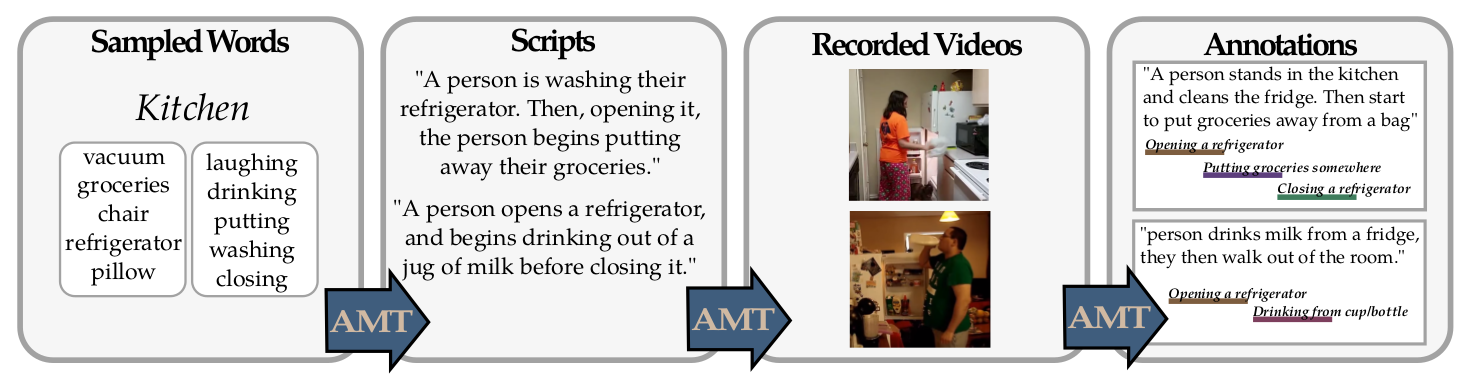
\includegraphics[width=\textwidth]{img_datasets/charades_amt_creation}
    \caption{Processing stages to create the Charades datset. \texttt{AMT} denotes the incorporation of worker from the Amazon Mechanical Turk service. \cite{sigurdsson_hollywood_2016}} 
    \label{fig:charades_amt_creation}
\end{figure}

Figure \ref{fig:charades_amt_creation} illustrates creation of the dataset in multiple stages:

\begin{enumerate}
    \item \textbf{Sampled Words \textrightarrow\  Scripts}\\
    By analyzing a total of 549 Movies focussing on the 15 most common indoor rooms of domestic households, the authors derived a list of 40 objects and 30 actions which occured most often in these scenes. The names of five randomly selected objects, five randomly selected actions and one randomly selected room were given to an AMT worker to combine into realistic activities scripts, that could occur in this room.
\item \textbf{Scripts \textrightarrow\  Recorded Videos}\\
    The previously created activity scripts are given to AMT workers to act out and record the described series of actions in an approximately 30 seconds long video. Analyzing the previously created activity scipts, the most frequent (verb, proposition, noun) triplets could be grouped into 157 action classes.
\item \textbf{Recorded Videos \textrightarrow\  Annotations}\\
    AMT workers annotate the created videos in multiple ways: Short description of the observed actions in text, identification of the present action classes, temporal localizaiton of the observed action classes and identification of the present objects.
\end{enumerate}

This crowdsourcing-based approach results in 9,848 videos created by 267 different people over three continents.
In total, the datasets contains $66,500$ temporally localized individual action instances.
Thereby each video contains on average 6.8 videos.

Figure ~\ref{fig:charades_vs_youtube} shows example frames from the charades dataset in comparison to frames from YouTube videos.
It demonstrates the atypical and entertaining nature of examples for action classes on YouTube.

\begin{figure}[H]
    \centering
    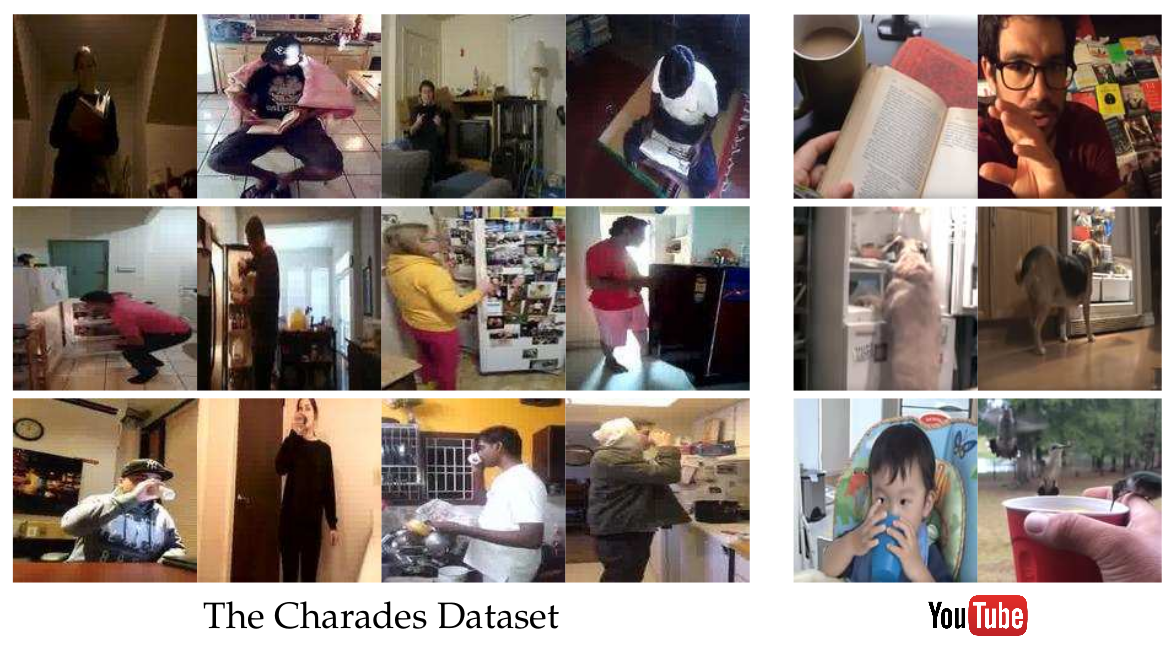
\includegraphics[width=\textwidth]{img_datasets/charades_vs_youtube}
    \caption{Rows show example frames of the actions \textit{reading}, \textit{opening fridge} and \textit{drinking}. Left: Frames from videos in the charades dataset. Right: Frames from sampled YouTube-videos. This illustrates the bias of YouTube videos towards entertaining actions and unrealistic settings. \cite{sigurdsson_hollywood_2016}}
    \label{fig:charades_vs_youtube}
\end{figure}

\subsubsection{Baseline Approaches on Charades}
\label{subsubsec:charades_baselines}

Additionally to releasing the dataset, several approaches for action recognition were implemented by the authors and evaluated on the Charades dataset.
These experimental results were obtained to provide baselines for comparing future approaches on the dataset.
The following approaches were implemented:

\begin{description}
    \item[Random] Presented with an input video, the classifier outputs a random action label.
    \item[C3D] The authors utilize the \textit{C3D} feature extractor introduced and published by \textcite{tran_learning_2015}. It is obtained by training a deep 3D convolutional network on the Sports-1M video dataset \cite{karpathy_large-scale_2014} and using the activations of the last convolutional network as a generic video-feature extractor. These features are then classified using one-versus-rest SVMs.
    \item[AlexNet] Deep 2D CNNs, AlexNet \cite{krizhevsky_imagenet_2012-1} and VGG-16 \cite{simonyan_very_2014} are being trained on a large collection of object images and extract frame-wise features over 30 equidistant frames of an input video. These features are averaged, normalized and then classified with one-versus-rest SVMs.
    \item[Two-Stream] The VGG-16 architecture is incorporated in a two-stream setup as introduced by \textcite{simonyan_two-stream_2014}. The spatial-stream network is pre-trained on ImageNet \cite{deng_imagenet:_2009} and the temporal-stream network is pre-trained on UCF-101 \cite{soomro_ucf101:_2012}. Both streams are then fine-tuned by training \textit{conv4}, \textit{conv5} and the fully-connected layers only.
    \item[Two-Stream-B] To handle class imbalance in the dataset, training of the previously described two-stream approach is adapted by ensuring that each training mini-batch of 256 examples contains at least 50 unique classes.
    \item[IDT] The authors implement the \textit{Improved Dense Trajectory (IDT)} approach \cite{wang_action_2013}, which relies on hand-crafted feature extractors. Spcifically MBH, HOG and HOF descriptors are being extracted around sampled trajectories in the input video. These descriptors are being encoded with Fisher Vectors \cite{perronnin_improving_2010}, which are then classified using one-versus-rest SVMs.
    \item[Combined] Represents the result of combining all previous approaches by late fusion \cite{karpathy_large-scale_2014}.
\end{description}

Because multiple action labels can be present per time-segment in a video of the dataset (see next section \ref{subsec:charadeslabelling}), the authors evaluate the perfomance of their implemented baseline approaches in terms of mean average precision (mAP).
For a discussion of mean average precision, which is a perfomance measure usually used in information retrieval, see appendix \ref{appendix:map}.
The results are shown in figure \ref{fig:charades_baseline_results}.

\begin{figure}[H]
    \centering
    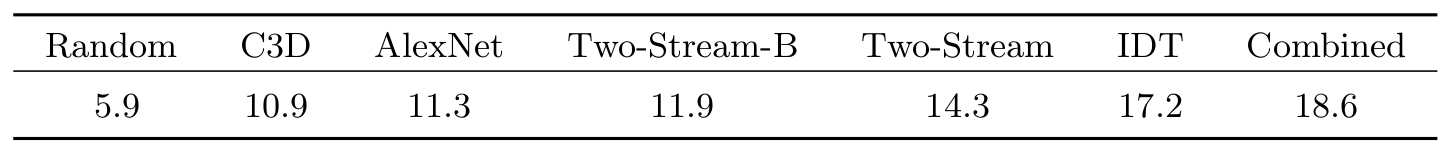
\includegraphics[width=\textwidth]{img_datasets/charades_baseline_results}
    \caption{Mean average precision of baseline approaches evaluated on the Charades dataset \cite{sigurdsson_hollywood_2016}}
    \label{fig:charades_baseline_results}
\end{figure}

\subsubsection{Recent Advances on Charades}

Alongside the publication, that describes the Charades dataset itself and the performance of various baseline approaches \cite{sigurdsson_hollywood_2016}, the authors additionally published an approach, proposing a fully-connected temporal Conditional Random Field (CRF) for action and intention recognition \cite{sigurdsson_asynchronous_2016}.
The incorporates various aspects of a human activity by modeling a video as a sequence of random variables, which capture the overall action category, present objects, the currently performed atomic action, the overall progress and the scene.
Human intention is incorporated as another unobserved latent variable.
For each frame in the input video, a two-stream CNN predicts the CRFs potentials.
The authors were thereby able to beat the baseline approaches by yielding an mAP of 22.4\%.

Accompanying the conference on Computer Vision and Pattern Recognition (CVPR) in July 2017, the Charades challenge for action recognition and action localization was posed.
Winner in both the localication and recognition track were TeamKinetics, lead by João Carreira, using their I3D approach \cite{carreira_quo_2017}.
Their approach yields 34.41\% mAP for action recognition with 29.74\% and 28.11\% being the second and third best results.
(Results obtained from \url{http://vuchallenge.org/charades.html})


\subsubsection{Labelling of the Charades Dataset}
\label{subsec:charadeslabelling}

The Charades dataset is richly labeled, in order to enable researcher to perform a variety of tasks on the dataset.
These tasks include scene/action/object recognition, action localization and action description.
The labels are provided in the form of comma separated values in two files (one for training, one for testing).
The example in table \ref{tab:example_labelling} corresponds to a single line in the training-labels file.

\begin{table}[H]
    \centering
    \texttt{
    \begin{tabularx}{\textwidth}{r X}
        id & RXLKF,\\
        subject & P6LJ,\\
        scene & Living room,\\
        quality & 4,\\
        relevance & 5,\\
        verified & Yes,\\
        script & A person is reading a book while snuggling on the sofa. They put the book down and begin standing while holding a cup of coffee,\\
        objects & blanket;book;coffee;couch;cup;glass;sofa;tissue,\\
        descriptions & "Person walks to couch wearing blanket, grabs book, place on lap, straighten blanket, opens book, reads it, closes book, place on couch, gets up, grabs tissue, clean face, place tissue back;The girl is walking to the couch with a blanket around her. She sits down, picks up a book, and begins reading. Then, she puts down the book and stands, takes a drink, puts it down, and walks back to the camera.",\\
        actions & c025 23.80 28.70;\newline c028 25.50 30.20;\newline c106 29.50 36.30;\newline c026 4.30 30.20;\newline c029 15.00 26.20;\newline c032 6.40 28.70;\newline c107 27.00 37.30;\newline c070 0.00 39.00;\newline c027 5.40 15.20;\newline c030 0.00 3.30;\newline c123 1.80 9.40;\newline c110 27.00 32.70;\newline c109 27.60 32.70;\newline c151 2.60 9.20;\newline c072 0.00 4.10,\\
        length & 38.08\\
    \end{tabularx}
    }
    \caption{Example labelling for a video of the training-set in the Charades dataset. \cite{sigurdsson_hollywood_2016}}
    \label{tab:example_labelling}
\end{table} 

The Charades dataset is available for download in different resolutions ($480$p and original resolution as provided by the AMT workers), decoded as RGB-frames and as optical flow images.
The different versions of the dataset are directly available for download at

\begin{center}
\url{http://allenai.org/plato/charades/}
\end{center}

Annotations and evaluation scripts in MATLAB to calculate the mean average precision (mAP) for the outputs of a model are provided as well.
We note, that this form of providing the dataset is most comfortable, as it is not needed to download individual videos from YouTube as with ActivityNet ??, Kinetics ?? and YouTube-8M.

The documentation of the dataset describes the individual fields of the annotations as follows:
\begin{table}[H]
    \centering
    \begin{tabularx}{\textwidth}{r X}
        \texttt{id} & Is a unique identifier for each video.\\
        \texttt{subject} & Describes an unique identifier for each subject, i.e. the person performing the action, in the dataset\\
        \texttt{scene} & One of the 15 domestic indoor scenes, i.e. rooms in the dataset. Examples are kitchen, dining room, living room or basement.\\
        \texttt{quality} & Indicates the quality of the video judged by an AMT annotator (7-point scale, 7=high quality).\\
        \texttt{relevance} & Indicates the relevance of the video to the script judged by an AMT annotator (7-point scale, 7=very relevant).\\
        \texttt{verified} & Describes if an annotator successfully verified that the video matches the script.\\
        \texttt{script} & The human-generated script, given to AMT workers to generate the video.\\
        \texttt{descriptions} & Semicolon-separated list of descriptions by annotators watching the video.\\
        \texttt{actions} & Semicolon-separated list of (class,start,end) triples for each action in the video. For example in table \ref{tab:example_labelling}: \texttt{c025} describes the action \textit{closing a book}, which lasts from second \texttt{23.80} to second \texttt{28.70} in the video.\\
        \texttt{length} & The length of the video in seconds.\\
    \end{tabularx}
    \caption{Descriptions of fields in the video annotations for the Charades dataset \cite{sigurdsson_hollywood_2016}}
    \label{tab:annotations_explained}
\end{table}

As can be seen in table \ref{tab:example_labelling}, annotated actions may overlap in videos of the charades dataset.
This is due to the facts, that humans are able to multitask and some actions naturally happen concurrently such as \textit{sitting on a chair} and \textit{working at a table}.
In this sense, the Charades dataset deviates from general action recognition benchmarking datasets, such as UCF-101 ?? HMDB-51 ?? and kinetics ??.
These provide unambiguous video clips, which are labelled with a single action to be recognised.
Charades is therefore more realistic, by providing less but longer video-files that contain multiple actions which can overlap.

Input video-clips for training a classifier can therefore be labelled in different ways: Either by providing only a single label with each input clip (one-hot-encoding) or by providing multiple lables for each clip (n-hot-encoding).
The latter would result from sampling an input clip from a region of overlapping actions. 

Multiple labels being possible for the same input clip results in a challenge when evaluating the performance of the network, since usually only a single output (the one with the biggest activation value) is taken as the network's prediction.
Therefore simply calculating the classifiers accuracy with a single target label per input is not an adequate measure of performance any more.
The mean average precision was therefore established as the standard performance measure on the dataset (see appendix \ref{appendix:map}).
